% ===== Section 4: "Crosswords don't actually keep your brain sharp" (~15 min) =====
\topicopener{puzzle}{Ուղեղի մարզում}{Խաչբառերը ուղեղդ սուր չեն պահում}{Ինչու է այդքան դժվար ուժեղացնել ուղեղը}{thinking}

% Looking clever vs becoming clever; the generator joke; poll
\begin{frame}{Խելացի երևալ, թե՞ խելացի դառնալ}
  \begin{columns}[T]
    \begin{column}{0.54\textwidth}
      Խելացի \textbf{երևալը} հեշտ է. ամպագոռգոռ բառեր («au courant»), ձեռքիդ՝ The Economist ամսագիրը։ Բայց կարելի՞ է իսկապես \textbf{դառնալ} ավելի խելացի։\par\medskip
      \onslide<2->{%
      \begin{bookquote}
        Ուղեղիդ էներգիան կարող ես մեծացնել՝ գլխով արդյունաբերական գեներատորի շղթան փակելով։ Միտքդ բառացիորեն կպայթի։ \emoji{exploding}
      \end{bookquote}}
    \end{column}
    \begin{column}{0.4\textwidth}
      \onslide<3->{%
      \begin{poll}
        Բարձրացրու ձեռքդ, եթե խաղացել ես «ուղեղի մարզման» հավելված։
      \end{poll}}
      \onslide<4->{%
      \begin{card}[colback=brainpink!25!cardwhite]
        Եթե դրանք աշխատեին, բոլորս հանճար կլինեինք, ու մեր ծանր գանգերը մեզ կճզմեին։
      \end{card}}
    \end{column}
  \end{columns}
\end{frame}

% How fMRI works
\begin{frame}{Ինչպես է աշխատում fMRI-ն}
  \begin{columns}[c]
    \begin{column}{0.5\textwidth}
      \begin{itemize}
        \item \textbf{Ֆունկցիոնալ ՄՌՏ} (fMRI). մարդը սկաների մեջ է, ու տեսնում ենք, թե ուղեղի որ մասն է աշխատում
        \item<2-> Աշխատող հյուսվածքին \textbf{թթվածին} է պետք։ Սկաները տարբերում է թթվածնով հարուստ ու աղքատ արյունը
        \item<3-> Բայց ուղեղը միշտ է ակտիվ, ու «ավելի ակտիվը» գտնելու համար շատ զտում ու վերլուծություն է պետք
      \end{itemize}
    \end{column}
    \begin{column}{0.46\textwidth}
      \centering
      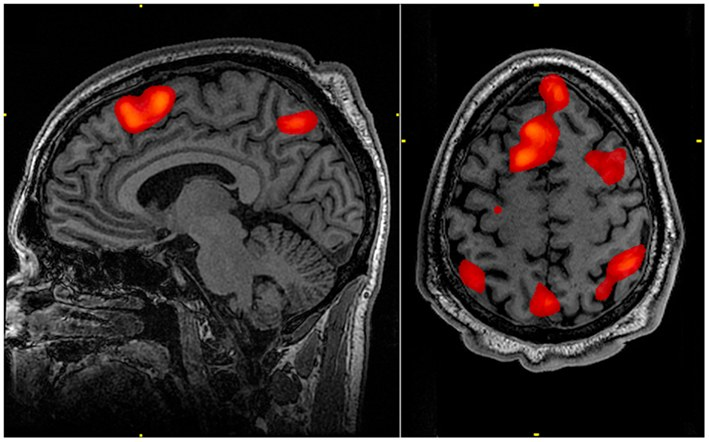
\includegraphics[width=\linewidth]{fmri_working_memory.jpg}\par\smallskip
      {\small fMRI. աշխատանքային հիշողության առաջադրանք։ Բըրնեթի «գունավոր բծերը» \emoji{grin}\par}
    \end{column}
  \end{columns}
\end{frame}

% Larson et al. 1995: clever brains work less
\begin{frame}{Լարսոնի տարօրինակ արդյունքը}
  \begin{columns}[c]
    \begin{column}{0.52\textwidth}
      \begin{itemize}
        \item Հեղուկ ինտելեկտի առաջադրանքներում նախաճակատային կեղևը ակտիվանում էր... \textbf{բացի նրանցից, ով շատ լավն էր}
        \item<2-> Ինչպես կշռել մարդկանց ու տեսնել, որ կշեռքը միայն թեթևներին է «տեսնում»
        \item<3-> Պարզվեց՝ խելացիների կեղևն էլ է ակտիվանում, բայց միայն երբ խնդիրը \textbf{իրենց համար} դժվար է
      \end{itemize}
    \end{column}
    \begin{column}{0.44\textwidth}
      \centering
      \onslide<3->{%
      \begin{tikzpicture}
        \node (a) at (0,0) {\mascot[1.9cm]{happy}};
        \node (b) at (3.0,0) {\mascot[1.9cm]{panic}};
        \node[font=\small, text=plum, align=center, anchor=north] at (a.south) {քեզ համար\\ \textbf{հեշտ է}};
        \node[font=\small, text=plum, align=center, anchor=north] at (b.south) {քեզ համար\\ \textbf{դժվար է}};
        \node[font=\scriptsize, text=mintdark, anchor=south] at (a.north) {կեղևը հանգիստ է};
        \node[font=\scriptsize, text=pinkdark, anchor=south] at (b.north) {կեղևը «վառվում» է};
      \end{tikzpicture}}
    \end{column}
  \end{columns}
  \source{Larson et al., Intelligence, 1995}
\end{frame}

% Efficiency beats power
\begin{frame}{Աղմկոտ շարժիչը լավագույնը չէ}
  \begin{columns}[c]
    \begin{column}{0.54\textwidth}
      \begin{itemize}
        \item Խելքը մեկ գոտու գործ չէ, այլ մի քանի \textbf{փոխկապակցված} գոտիների՝ նախաճակատային կեղևի, գագաթային բլթի և այլն
        \item<2-> Խելացի մարդկանց մոտ այդ կապերն ավելի \textbf{արդյունավետ} են, ու ընդհանուր ակտիվությունը՝ ավելի քիչ
        \item<3-> Որքան լավ են մասերը «խոսում» իրար հետ, այնքան արագ ու հեշտ են որոշումներն ու հաշվարկները
      \end{itemize}
    \end{column}
    \begin{column}{0.4\textwidth}
      \centering
      \bigemoji[1.2cm]{car}\ \bigemoji[0.9cm]{loudspeaker}\ \bigemoji[0.9cm]{fire}\par\smallskip
      \begin{bookquote}
        Մեքենան, որի շարժիչը մռնչում է առյուծների ոհմակի պես, որը փոթորիկ է ձևացնում, պարտադիր չէ, որ անաղմուկից լավը լինի։
      \end{bookquote}
    \end{column}
  \end{columns}
\end{frame}

% White matter: the roads
\begin{frame}{Սպիտակ նյութը՝ ճանապարհներ}
  \begin{columns}[c]
    \begin{column}{0.54\textwidth}
      \begin{itemize}
        \item \textbf{Գորշ նյութ} (grey matter)՝ որտեղ ակտիվությունն է ստեղծվում. «գործարանները»
        \item<2-> \textbf{Սպիտակ նյութ} (white matter)՝ նեյրոնների երկար «լարերի» (աքսոնների) կապոցներ. «ճանապարհները»։ Ուղեղի մոտ \textbf{կեսն} է
        \item<3-> Սպիտակ նյութի ամբողջականությունն ու խտությունը խելքի \textbf{հուսալի ցուցիչ} են
      \end{itemize}
    \end{column}
    \begin{column}{0.4\textwidth}
      \centering
      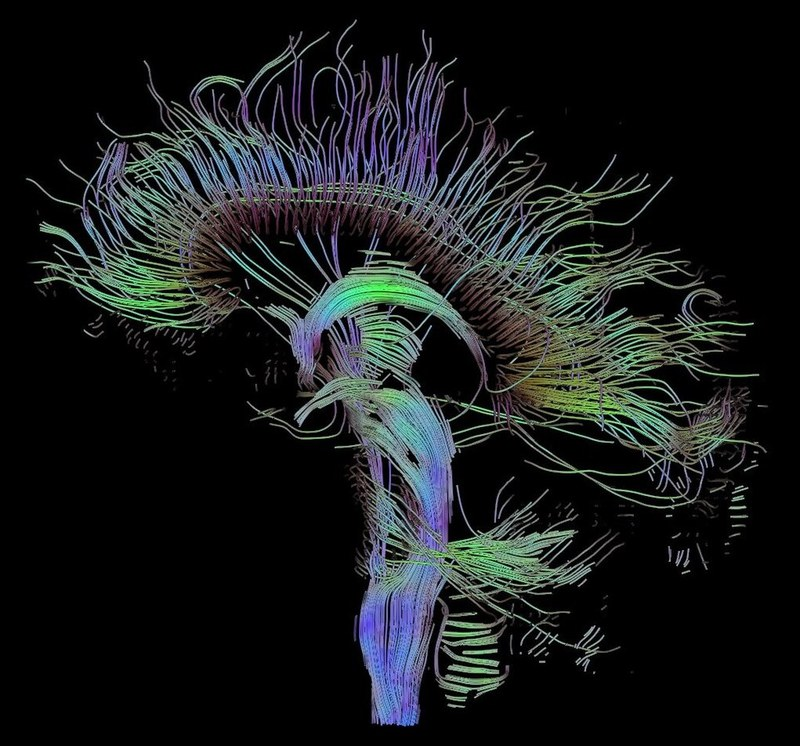
\includegraphics[width=0.85\linewidth]{dti_white_matter.jpg}\par\smallskip
      {\small Սպիտակ նյութի «ճանապարհները» (DTI տրակտոգրաֆիա)\par}
    \end{column}
  \end{columns}
\end{frame}

% Corpus callosum; needle joke; consoles
\begin{frame}{Կամուրջ կիսագնդերի միջև}
  \begin{columns}[T]
    \begin{column}{0.5\textwidth}
      \begin{itemize}
        \item Որքան լավ են կապերը, այնքան քիչ էներգիա է պետք, ու այնքան \textbf{դժվար է} դրանք սկաներով գտնել
        \item<2-> \textbf{Corpus callosum}՝ սպիտակ նյութի մեծ «կամուրջը» կիսագնդերի միջև։ Որքան հաստ է, այնքան լավ են նրանք «խոսում», ու դա կապված է ընդհանուր խելքի հետ
      \end{itemize}
    \end{column}
    \begin{column}{0.44\textwidth}
      \begin{bookquote}
        Ինչպես ասեղ փնտրել դեզում, որն ավելի մեծ ասեղների կույտ է, ու այն էլ՝ լվացքի մեքենայում։
      \end{bookquote}
      \onslide<3->{%
      \begin{card}[colback=mint!35!cardwhite]
        \emoji[1.3em]{videogame}\ Տարբեր կառուցվածքով ուղեղները կարող են նույնքան խելացի լինել. ինչպես տարբեր ֆիրմաների կոնսոլները։
      \end{card}}
    \end{column}
  \end{columns}
\end{frame}

% Learning does change the brain
\begin{frame}{Ուրեմն ինչպե՞ս դառնալ ավելի խելացի}
  \begin{columns}[T]
    \begin{column}{0.52\textwidth}
      \begin{itemize}
        \item Ակնհայտ պատասխանը՝ \textbf{սովորել}։ Ամեն նոր փաստ մեծացնում է բյուրեղացած ինտելեկտը
        \item<2-> Հեղուկ ինտելեկտը կիրառիր որքան հնարավոր է շատ տարբեր իրավիճակներում
        \item<3-> Ուղեղը \textbf{պլաստիկ} է. փոխվում է պահանջներին համապատասխան. նոր հիշողությունը նոր սինապսներ է (գլուխ 2)
      \end{itemize}
    \end{column}
    \begin{column}{0.44\textwidth}
      \onslide<4->{%
      \begin{scienceupdate}
        2018-ի մեծ վերլուծությունը (42 տվյալների բազա, 600 000+ մարդ). ամեն լրացուցիչ \textbf{տարվա կրթությունը} IQ-ն բարձրացնում է \textbf{մոտ 1-5 միավորով} (միջինը՝ մոտ 3.4)։
      \end{scienceupdate}}
    \end{column}
  \end{columns}
  \source{Ritchie \& Tucker-Drob, Psychological Science, 2018}
\end{frame}

% Musicians' hands: the motor cortex
\begin{frame}{Երաժիշտների ձեռքերը}
  \begin{columns}[c]
    \begin{column}{0.56\textwidth}
      \begin{itemize}
        \item \textbf{Շարժողական կեղևը} (motor cortex) ղեկավարում է կամային շարժումները. մարմնի ամեն մաս ունի իր «տարածքը»
        \item<2-> Իրանը քիչ տեղ ունի, իսկ դեմքն ու ձեռքերը՝ շատ. դրանք նուրբ կառավարում են պահանջում
        \item<3-> Ջութակահարների ու դաշնակահարների մոտ մատների «տարածքը» \textbf{ավելի մեծ է}. ուղեղը հարմարվել է
      \end{itemize}
      \vspace{1mm}
      {\scriptsize\emoji{microscope}\ Գրքում՝ «գագաթային բլթում»։ Իրականում շարժողական կեղևը \textbf{ճակատային} բլթի հետին մասն է։\par}
    \end{column}
    \begin{column}{0.4\textwidth}
      \centering
      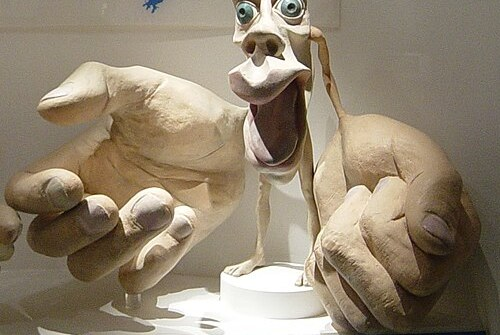
\includegraphics[width=0.92\linewidth]{motor_homunculus.jpg}\par\smallskip
      {\small Այսպիսին կլինեիր, եթե մարմնի ամեն մաս այնքան մեծ լիներ, որքան կեղևում նրա «տարածքը» (շարժողական «հոմունկուլուս»)\par}
    \end{column}
  \end{columns}
\end{frame}

% Taxi drivers and mice
\begin{frame}{Տաքսու վարորդներն ու մկները}
  \begin{columns}[c]
    \begin{column}{0.56\textwidth}
      \begin{itemize}
        \item Լոնդոնի տաքսու վարորդները պետք է անգիր իմանան քաղաքի խճճված փողոցները («the Knowledge»)։ Նրանց \textbf{հիպոկամպի հետին մասը} ավելի մեծ էր
        \item<2-> Դա GPS-ից առաջ էր։ Ով գիտի, ինչ կլիներ այսօր
        \item<3-> Մկների փորձերում նոր հմտություն սովորելը ամրացնում է սպիտակ նյութը՝ հաստացնելով \textbf{միելինը} (նյարդաթելի «մեկուսիչ» շերտը)
      \end{itemize}
    \end{column}
    \begin{column}{0.38\textwidth}
      \centering
      \bigemoji[1.3cm]{taxi}\ \bigemoji[1.3cm]{mouse}\par\medskip
      \onslide<3->{%
      \begin{bookquote}
        Մկներ, իսկ նրանք որքա՞ն կարող են խելացի լինել...
      \end{bookquote}}
      \onslide<4->{\small Ուրեմն, տեխնիկապես, ուղեղի «ուժը» մեծացնելու ձևեր կան։\par}
    \end{column}
  \end{columns}
  \source{Maguire et al., PNAS, 2000}
\end{frame}

% The bad news (+ science update on "brain finished at 25")
\begin{frame}{Իսկ հիմա՝ վատ լուրը}
  \begin{columns}[T]
    \begin{column}{0.54\textwidth}
      \begin{itemize}
        \item Սա \textbf{երկար ժամանակ ու ջանք} է պահանջում, իսկ արդյունքը սահմանափակ է
        \item<2-> Երաժիշտը նոտաներ լավ է կարդում, բայց մաթեմատիկայում դրանից չի լավանում
        \item<3-> Հեղուկ ինտելեկտը շատ կապերի արդյունք է, ու դժվար է այն «մարզել»
        \item<4-> Գրքի խոսքով՝ 25-ում ուղեղը ձևավորված է, ու մեծերի հեղուկ ինտելեկտը «ֆիքսված» է
      \end{itemize}
    \end{column}
    \begin{column}{0.42\textwidth}
      \onslide<5->{%
      \begin{scienceupdate}
        «25-ում ուղեղը պատրաստ է» պնդումը պարզեցում է։ 2025-ին 4000+ մարդու ուղեղի սկաները ցույց տվեցին, որ կապերի «դեռահասային» վերակառուցումը տևում է \textbf{մինչև մոտ 32 տարեկան}։
      \end{scienceupdate}}
    \end{column}
  \end{columns}
  \source{Mousley et al., Nature Communications, 2025}
\end{frame}

% Brain-training games (+ science update)
\begin{frame}{«Ուղեղի մարզման» խաղերը}
  \begin{columns}[T]
    \begin{column}{0.5\textwidth}
      \begin{itemize}
        \item Ընկերությունները վաճառում են գլուխկոտրուկներ, որոնք իբր բարձրացնում են խելքը
        \item<2-> Շատ խաղալով իսկապես լավանում ես... \textbf{միայն այդ խաղում}
        \item<3-> Ապացույց չկա, որ դրանք բարձրացնում են \textbf{ընդհանուր} խելքը. ուղեղը բավական բարդ է, որ մեկ խաղում լավանա՝ առանց մնացածը փոխելու
      \end{itemize}
    \end{column}
    \begin{column}{0.46\textwidth}
      \onslide<4->{%
      \begin{scienceupdate}
        2016-ի մեծ ակնարկը հաստատեց. մարզված առաջադրանքում լավանում ես, իսկ այլ խնդիրների վրա ազդեցությունը (far transfer) գրեթե չկա։\par\smallskip
        Նույն տարում Lumosity-ն ԱՄՆ-ում \textbf{2 միլիոն դոլար} վճարեց չհիմնավորված գովազդի համար։
      \end{scienceupdate}}
    \end{column}
  \end{columns}
  \source{Simons et al., Psychol. Sci. Public Interest, 2016; FTC, 2016}
\end{frame}

% Meme: Gru's plan, brain training
\begin{frame}{Կատարյալ պլան}
  \centering
  \begin{meme}[9.4cm]{gru_plan.jpg}
    \memecap[text width=1.8cm, font=\blackfont\footnotesize]{0.386}{0.74}{Ներբեռնում եմ «ուղեղի մարզիչ»}
    \memecap[text width=1.75cm, font=\blackfont\footnotesize]{0.885}{0.74}{Ամեն օր խաղում եմ մի ամիս}
    \memecap[text width=1.75cm, font=\blackfont\footnotesize]{0.386}{0.24}{Դառնում եմ հանճար}
    \memecap[text width=1.75cm, font=\blackfont\footnotesize]{0.885}{0.24}{Լավ եմ միայն այդ խաղում}
  \end{meme}
\end{frame}

% Study drugs and nootropics
\begin{frame}{Քննությունից առաջ՝ հաբե՞ր}
  \begin{columns}[T]
    \begin{column}{0.56\textwidth}
      \begin{itemize}
        \item Որոշ ուսանողներ քննությունից առաջ խմում են ADHD-ի դեղեր (Ռիտալին, Ադերալ)՝ կենտրոնանալու համար
        \item<2-> Օգուտը կարճ է, իսկ առանց ADHD-ի երկարաժամկետ վնասը կարող է \textbf{լուրջ} լինել
        \item<3-> Կարող է և խանգարել. ուժասպառ ես լինում ու \textbf{քնում ես հենց քննության ժամին} \emoji{sleeping}
        \item<4-> «Խելքի դեղերը» (nootropics) նոր են ու նեղ ազդեցություն ունեն
      \end{itemize}
    \end{column}
    \begin{column}{0.4\textwidth}
      \centering
      \bigemoji[1.0cm]{pill}\par\smallskip
      \onslide<5->{%
      \begin{scienceupdate}
        Առողջ երիտասարդների մոտ Ադերալը թեստերի արդյունքը գրեթե չփոխեց, բայց մասնակիցները \textbf{կարծում էին}, որ ավելի լավ են գրել։
      \end{scienceupdate}}
    \end{column}
  \end{columns}
  \source{Ilieva et al., Neuropharmacology, 2013}
\end{frame}

% Fish oil and tDCS
\begin{frame}{Ձկան յուղ ու հոսանք գլխին}
  \begin{columns}[T]
    \begin{column}{0.44\textwidth}
      \begin{itemize}
        \item \emoji{fish}\ «Խելքի սնունդը» (օր.՝ ձկան յուղ) կասկածելի է
        \item<2-> \emoji{lightning}\ tDCS՝ թույլ հոսանք գանգի միջով։ 2014-ի ակնարկը որոշ լավացում գտավ, այլոք՝ ոչ
        \item<3-> Իսկ tDCS սարքեր արդեն վաճառում են՝ խաղերում «լավանալու» համար
      \end{itemize}
    \end{column}
    \begin{column}{0.52\textwidth}
      \onslide<4->{%
      \begin{bookquote}
        Նույնն է, թե հակադեպրեսանտներ վաճառես շոկոլադների կողքին։
      \end{bookquote}}
      \onslide<5->{%
      \begin{scienceupdate}
        2015-ի մեծ ակնարկ. մեկ սեանսը առողջների մտածողությունը \textbf{հուսալիորեն չի փոխում}։
      \end{scienceupdate}}
    \end{column}
  \end{columns}
  \source{Bennabi et al., 2014; Horvath et al., Brain Stimulation, 2015}
\end{frame}

% Conclusion of the section
\begin{frame}{Ուրեմն կարելի՞ է խելացի դառնալ}
  \begin{columns}[c]
    \begin{column}{0.54\textwidth}
      \begin{itemize}
        \item \textbf{Այո}, բայց երկար ժամանակ ու համառ ջանքով
        \item<2-> Միայն այն անելը, ինչում արդեն լավն ես, չի օգնի։ Երբ ինչ-որ բան շատ լավ ես անում, ուղեղն այնքան արդյունավետ է դառնում, որ \textbf{չի էլ նկատում} այն ու չի փոխվում
        \item<3-> Դրա համար էլ հազարերորդ խաչբառը քեզ չի «սրում» \emoji{puzzle}
      \end{itemize}
    \end{column}
    \begin{column}{0.4\textwidth}
      \centering
      \onslide<4->{%
      \mascot[1.8cm]{smug}\par\smallskip
      \begin{bookquote}
        Ավելի խելացի դառնալու համար պետք է կա՛մ շատ համառ լինես, կա՛մ շատ խելացի, որ խորամանկես սեփական ուղեղիդ։
      \end{bookquote}}
    \end{column}
  \end{columns}
\end{frame}
